% Options for packages loaded elsewhere
\PassOptionsToPackage{unicode}{hyperref}
\PassOptionsToPackage{hyphens}{url}
%
\documentclass[
]{article}
\usepackage{amsmath,amssymb}
\usepackage{iftex}
\ifPDFTeX
  \usepackage[T1]{fontenc}
  \usepackage[utf8]{inputenc}
  \usepackage{textcomp} % provide euro and other symbols
\else % if luatex or xetex
  \usepackage{unicode-math} % this also loads fontspec
  \defaultfontfeatures{Scale=MatchLowercase}
  \defaultfontfeatures[\rmfamily]{Ligatures=TeX,Scale=1}
\fi
\usepackage{lmodern}
\ifPDFTeX\else
  % xetex/luatex font selection
\fi
% Use upquote if available, for straight quotes in verbatim environments
\IfFileExists{upquote.sty}{\usepackage{upquote}}{}
\IfFileExists{microtype.sty}{% use microtype if available
  \usepackage[]{microtype}
  \UseMicrotypeSet[protrusion]{basicmath} % disable protrusion for tt fonts
}{}
\makeatletter
\@ifundefined{KOMAClassName}{% if non-KOMA class
  \IfFileExists{parskip.sty}{%
    \usepackage{parskip}
  }{% else
    \setlength{\parindent}{0pt}
    \setlength{\parskip}{6pt plus 2pt minus 1pt}}
}{% if KOMA class
  \KOMAoptions{parskip=half}}
\makeatother
\usepackage{xcolor}
\usepackage[margin=1in]{geometry}
\usepackage{color}
\usepackage{fancyvrb}
\newcommand{\VerbBar}{|}
\newcommand{\VERB}{\Verb[commandchars=\\\{\}]}
\DefineVerbatimEnvironment{Highlighting}{Verbatim}{commandchars=\\\{\}}
% Add ',fontsize=\small' for more characters per line
\usepackage{framed}
\definecolor{shadecolor}{RGB}{248,248,248}
\newenvironment{Shaded}{\begin{snugshade}}{\end{snugshade}}
\newcommand{\AlertTok}[1]{\textcolor[rgb]{0.94,0.16,0.16}{#1}}
\newcommand{\AnnotationTok}[1]{\textcolor[rgb]{0.56,0.35,0.01}{\textbf{\textit{#1}}}}
\newcommand{\AttributeTok}[1]{\textcolor[rgb]{0.13,0.29,0.53}{#1}}
\newcommand{\BaseNTok}[1]{\textcolor[rgb]{0.00,0.00,0.81}{#1}}
\newcommand{\BuiltInTok}[1]{#1}
\newcommand{\CharTok}[1]{\textcolor[rgb]{0.31,0.60,0.02}{#1}}
\newcommand{\CommentTok}[1]{\textcolor[rgb]{0.56,0.35,0.01}{\textit{#1}}}
\newcommand{\CommentVarTok}[1]{\textcolor[rgb]{0.56,0.35,0.01}{\textbf{\textit{#1}}}}
\newcommand{\ConstantTok}[1]{\textcolor[rgb]{0.56,0.35,0.01}{#1}}
\newcommand{\ControlFlowTok}[1]{\textcolor[rgb]{0.13,0.29,0.53}{\textbf{#1}}}
\newcommand{\DataTypeTok}[1]{\textcolor[rgb]{0.13,0.29,0.53}{#1}}
\newcommand{\DecValTok}[1]{\textcolor[rgb]{0.00,0.00,0.81}{#1}}
\newcommand{\DocumentationTok}[1]{\textcolor[rgb]{0.56,0.35,0.01}{\textbf{\textit{#1}}}}
\newcommand{\ErrorTok}[1]{\textcolor[rgb]{0.64,0.00,0.00}{\textbf{#1}}}
\newcommand{\ExtensionTok}[1]{#1}
\newcommand{\FloatTok}[1]{\textcolor[rgb]{0.00,0.00,0.81}{#1}}
\newcommand{\FunctionTok}[1]{\textcolor[rgb]{0.13,0.29,0.53}{\textbf{#1}}}
\newcommand{\ImportTok}[1]{#1}
\newcommand{\InformationTok}[1]{\textcolor[rgb]{0.56,0.35,0.01}{\textbf{\textit{#1}}}}
\newcommand{\KeywordTok}[1]{\textcolor[rgb]{0.13,0.29,0.53}{\textbf{#1}}}
\newcommand{\NormalTok}[1]{#1}
\newcommand{\OperatorTok}[1]{\textcolor[rgb]{0.81,0.36,0.00}{\textbf{#1}}}
\newcommand{\OtherTok}[1]{\textcolor[rgb]{0.56,0.35,0.01}{#1}}
\newcommand{\PreprocessorTok}[1]{\textcolor[rgb]{0.56,0.35,0.01}{\textit{#1}}}
\newcommand{\RegionMarkerTok}[1]{#1}
\newcommand{\SpecialCharTok}[1]{\textcolor[rgb]{0.81,0.36,0.00}{\textbf{#1}}}
\newcommand{\SpecialStringTok}[1]{\textcolor[rgb]{0.31,0.60,0.02}{#1}}
\newcommand{\StringTok}[1]{\textcolor[rgb]{0.31,0.60,0.02}{#1}}
\newcommand{\VariableTok}[1]{\textcolor[rgb]{0.00,0.00,0.00}{#1}}
\newcommand{\VerbatimStringTok}[1]{\textcolor[rgb]{0.31,0.60,0.02}{#1}}
\newcommand{\WarningTok}[1]{\textcolor[rgb]{0.56,0.35,0.01}{\textbf{\textit{#1}}}}
\usepackage{longtable,booktabs,array}
\usepackage{calc} % for calculating minipage widths
% Correct order of tables after \paragraph or \subparagraph
\usepackage{etoolbox}
\makeatletter
\patchcmd\longtable{\par}{\if@noskipsec\mbox{}\fi\par}{}{}
\makeatother
% Allow footnotes in longtable head/foot
\IfFileExists{footnotehyper.sty}{\usepackage{footnotehyper}}{\usepackage{footnote}}
\makesavenoteenv{longtable}
\usepackage{graphicx}
\makeatletter
\def\maxwidth{\ifdim\Gin@nat@width>\linewidth\linewidth\else\Gin@nat@width\fi}
\def\maxheight{\ifdim\Gin@nat@height>\textheight\textheight\else\Gin@nat@height\fi}
\makeatother
% Scale images if necessary, so that they will not overflow the page
% margins by default, and it is still possible to overwrite the defaults
% using explicit options in \includegraphics[width, height, ...]{}
\setkeys{Gin}{width=\maxwidth,height=\maxheight,keepaspectratio}
% Set default figure placement to htbp
\makeatletter
\def\fps@figure{htbp}
\makeatother
\setlength{\emergencystretch}{3em} % prevent overfull lines
\providecommand{\tightlist}{%
  \setlength{\itemsep}{0pt}\setlength{\parskip}{0pt}}
\setcounter{secnumdepth}{-\maxdimen} % remove section numbering
\ifLuaTeX
  \usepackage{selnolig}  % disable illegal ligatures
\fi
\IfFileExists{bookmark.sty}{\usepackage{bookmark}}{\usepackage{hyperref}}
\IfFileExists{xurl.sty}{\usepackage{xurl}}{} % add URL line breaks if available
\urlstyle{same}
\hypersetup{
  pdftitle={Homework 1},
  pdfauthor={Group M: Billo, Pizzignacco, El Gataa, Shahzad},
  hidelinks,
  pdfcreator={LaTeX via pandoc}}

\title{Homework 1}
\author{Group M: Billo, Pizzignacco, El Gataa, Shahzad}
\date{}

\begin{document}
\maketitle

\hypertarget{introduction}{%
\subsection{Introduction}\label{introduction}}

\emph{Briefly describe the purpose of the homework or tasks to be
accomplished.}

\hypertarget{block-b}{%
\subsection{Block B}\label{block-b}}

\hypertarget{cs-chapter-1-exercises-1.1-1.6}{%
\subsubsection{CS: Chapter 1, exercises 1.1,
1.6}\label{cs-chapter-1-exercises-1.1-1.6}}

\begin{Shaded}
\begin{Highlighting}[]
\CommentTok{\# Placeholder for code for Exercise B1}
\end{Highlighting}
\end{Shaded}

\hypertarget{cs-chapter-3}{%
\subsubsection{CS: Chapter 3}\label{cs-chapter-3}}

exercises 3.5

\begin{Shaded}
\begin{Highlighting}[]
\CommentTok{\# Ax = y}
\FunctionTok{set.seed}\NormalTok{(}\DecValTok{0}\NormalTok{)}
\NormalTok{n }\OtherTok{\textless{}{-}} \DecValTok{1000}
\NormalTok{A }\OtherTok{\textless{}{-}} \FunctionTok{matrix}\NormalTok{(}\FunctionTok{runif}\NormalTok{(n }\SpecialCharTok{*}\NormalTok{ n), n, n)}
\NormalTok{x.true }\OtherTok{\textless{}{-}} \FunctionTok{runif}\NormalTok{(n)}
\NormalTok{y }\OtherTok{\textless{}{-}}\NormalTok{ A }\SpecialCharTok{\%*\%}\NormalTok{ x.true}

\CommentTok{\# b)}

\NormalTok{start\_time }\OtherTok{\textless{}{-}} \FunctionTok{Sys.time}\NormalTok{()}
\NormalTok{A\_inv }\OtherTok{\textless{}{-}} \FunctionTok{solve}\NormalTok{(A)}
\NormalTok{x1 }\OtherTok{\textless{}{-}}\NormalTok{ A\_inv }\SpecialCharTok{\%*\%}\NormalTok{ y}
\NormalTok{end\_time }\OtherTok{\textless{}{-}} \FunctionTok{Sys.time}\NormalTok{()}
\NormalTok{time\_taken }\OtherTok{\textless{}{-}}\NormalTok{ end\_time }\SpecialCharTok{{-}}\NormalTok{ start\_time}

\CommentTok{\# Calculate the mean absolute error}
\NormalTok{mean\_absolute\_error }\OtherTok{\textless{}{-}} \FunctionTok{mean}\NormalTok{(}\FunctionTok{abs}\NormalTok{(x1 }\SpecialCharTok{{-}}\NormalTok{ x.true))}

\FunctionTok{print}\NormalTok{(time\_taken)}
\end{Highlighting}
\end{Shaded}

\begin{verbatim}
## Time difference of 0.2257133 secs
\end{verbatim}

\begin{Shaded}
\begin{Highlighting}[]
\FunctionTok{print}\NormalTok{(mean\_absolute\_error)}
\end{Highlighting}
\end{Shaded}

\begin{verbatim}
## [1] 2.560437e-11
\end{verbatim}

\begin{Shaded}
\begin{Highlighting}[]
\CommentTok{\# c)}
\NormalTok{start\_time\_direct }\OtherTok{\textless{}{-}} \FunctionTok{Sys.time}\NormalTok{()}
\NormalTok{x2 }\OtherTok{\textless{}{-}} \FunctionTok{solve}\NormalTok{(A, y)}
\NormalTok{end\_time\_direct }\OtherTok{\textless{}{-}} \FunctionTok{Sys.time}\NormalTok{()}
\NormalTok{time\_taken\_direct }\OtherTok{\textless{}{-}}\NormalTok{ end\_time\_direct }\SpecialCharTok{{-}}\NormalTok{ start\_time\_direct}

\CommentTok{\# Calculate the mean absolute error}
\NormalTok{mean\_absolute\_error\_direct }\OtherTok{\textless{}{-}} \FunctionTok{mean}\NormalTok{(}\FunctionTok{abs}\NormalTok{(x2 }\SpecialCharTok{{-}}\NormalTok{ x.true))}

\FunctionTok{print}\NormalTok{(time\_taken\_direct)}
\end{Highlighting}
\end{Shaded}

\begin{verbatim}
## Time difference of 0.2156529 secs
\end{verbatim}

\begin{Shaded}
\begin{Highlighting}[]
\FunctionTok{print}\NormalTok{(mean\_absolute\_error\_direct)}
\end{Highlighting}
\end{Shaded}

\begin{verbatim}
## [1] 7.801055e-13
\end{verbatim}

\begin{Shaded}
\begin{Highlighting}[]
\CommentTok{\# d) Conclusion:}

\CommentTok{\# Calculate time to explicitly form the inverse matrix A\^{}{-}1 and solve Ax = y}
\NormalTok{start\_time }\OtherTok{\textless{}{-}} \FunctionTok{Sys.time}\NormalTok{()}
\NormalTok{A\_inv }\OtherTok{\textless{}{-}} \FunctionTok{solve}\NormalTok{(A)}
\NormalTok{x1 }\OtherTok{\textless{}{-}}\NormalTok{ A\_inv }\SpecialCharTok{\%*\%}\NormalTok{ y}
\NormalTok{end\_time }\OtherTok{\textless{}{-}} \FunctionTok{Sys.time}\NormalTok{()}
\NormalTok{time\_taken }\OtherTok{\textless{}{-}}\NormalTok{ end\_time }\SpecialCharTok{{-}}\NormalTok{ start\_time}

\CommentTok{\# Calculate the mean absolute error between x1 and x.true}
\NormalTok{mean\_absolute\_error }\OtherTok{\textless{}{-}} \FunctionTok{mean}\NormalTok{(}\FunctionTok{abs}\NormalTok{(x1 }\SpecialCharTok{{-}}\NormalTok{ x.true))}

\FunctionTok{print}\NormalTok{(time\_taken)}
\end{Highlighting}
\end{Shaded}

\begin{verbatim}
## Time difference of 0.1736169 secs
\end{verbatim}

\begin{Shaded}
\begin{Highlighting}[]
\FunctionTok{print}\NormalTok{(mean\_absolute\_error)}
\end{Highlighting}
\end{Shaded}

\begin{verbatim}
## [1] 2.560437e-11
\end{verbatim}

\begin{Shaded}
\begin{Highlighting}[]
\CommentTok{\# Calculate time to directly solve Ax = y without forming A\^{}{-}1}
\NormalTok{start\_time\_direct }\OtherTok{\textless{}{-}} \FunctionTok{Sys.time}\NormalTok{()}
\NormalTok{x2 }\OtherTok{\textless{}{-}} \FunctionTok{solve}\NormalTok{(A, y)}
\NormalTok{end\_time\_direct }\OtherTok{\textless{}{-}} \FunctionTok{Sys.time}\NormalTok{()}
\NormalTok{time\_taken\_direct }\OtherTok{\textless{}{-}}\NormalTok{ end\_time\_direct }\SpecialCharTok{{-}}\NormalTok{ start\_time\_direct}

\CommentTok{\# Calculate the mean absolute error between x2 and x.true}
\NormalTok{mean\_absolute\_error\_direct }\OtherTok{\textless{}{-}} \FunctionTok{mean}\NormalTok{(}\FunctionTok{abs}\NormalTok{(x2 }\SpecialCharTok{{-}}\NormalTok{ x.true))}

\FunctionTok{print}\NormalTok{(time\_taken\_direct)}
\end{Highlighting}
\end{Shaded}

\begin{verbatim}
## Time difference of 0.09286594 secs
\end{verbatim}

\begin{Shaded}
\begin{Highlighting}[]
\FunctionTok{print}\NormalTok{(mean\_absolute\_error\_direct)}
\end{Highlighting}
\end{Shaded}

\begin{verbatim}
## [1] 7.801055e-13
\end{verbatim}

Conclusion: Using `solve' to directly solve the equation Ax = y is
significantly faster (approximately 0.39 seconds) compared to explicitly
forming A\^{}-1 and then multiplying it by y (approximately 2.29
seconds).

While both solutions are very precise, directly solving with `solve'
yields a slightly smaller mean absolute error (approximately 1.36e-12)
compared to forming the inverse (approximately 2.96e-11).

Therefore, solving the linear system directly without calculating the
explicit inverse is preferable in terms of both efficiency and accuracy.

es 3.6

\begin{Shaded}
\begin{Highlighting}[]
\CommentTok{\# a)}
\CommentTok{\# Function to calculate the ECDF}
\NormalTok{ecdf\_values }\OtherTok{\textless{}{-}} \ControlFlowTok{function}\NormalTok{(x) \{}
  \CommentTok{\# Total number of observations}
\NormalTok{  n }\OtherTok{\textless{}{-}} \FunctionTok{length}\NormalTok{(x)}
  
  \CommentTok{\# Sort x values with sort.int, keeping the original indices}
\NormalTok{  sorted\_x }\OtherTok{\textless{}{-}} \FunctionTok{sort.int}\NormalTok{(x, }\AttributeTok{index.return =} \ConstantTok{TRUE}\NormalTok{)}
  
  \CommentTok{\# Calculate the ECDF for each value in x}
\NormalTok{  ecdf }\OtherTok{\textless{}{-}}\NormalTok{ (}\DecValTok{1}\SpecialCharTok{:}\NormalTok{n) }\SpecialCharTok{/}\NormalTok{ n}
  
  \CommentTok{\# Reorder the ECDF values to the original order}
\NormalTok{  ecdf\_original\_order }\OtherTok{\textless{}{-}}\NormalTok{ ecdf[}\FunctionTok{order}\NormalTok{(sorted\_x}\SpecialCharTok{$}\NormalTok{ix)]}
  
  \FunctionTok{return}\NormalTok{(ecdf\_original\_order)}
\NormalTok{\}}

\CommentTok{\# Test the function with an example}
\FunctionTok{set.seed}\NormalTok{(}\DecValTok{123}\NormalTok{)}
\NormalTok{x }\OtherTok{\textless{}{-}} \FunctionTok{rnorm}\NormalTok{(}\DecValTok{10}\NormalTok{)}
\FunctionTok{ecdf\_values}\NormalTok{(x)}
\end{Highlighting}
\end{Shaded}

\begin{verbatim}
##  [1] 0.3 0.5 0.9 0.6 0.7 1.0 0.8 0.1 0.2 0.4
\end{verbatim}

\begin{Shaded}
\begin{Highlighting}[]
\CommentTok{\# b)}
\CommentTok{\# Function to calculate the ECDF and optionally plot it}
\NormalTok{ecdf\_values }\OtherTok{\textless{}{-}} \ControlFlowTok{function}\NormalTok{(x, }\AttributeTok{plot.cdf =} \ConstantTok{FALSE}\NormalTok{) \{}
  \CommentTok{\# Total number of observations}
\NormalTok{  n }\OtherTok{\textless{}{-}} \FunctionTok{length}\NormalTok{(x)}
  
  \CommentTok{\# Sort x values}
\NormalTok{  sorted\_x }\OtherTok{\textless{}{-}} \FunctionTok{sort}\NormalTok{(x)}
  
  \CommentTok{\# Calculate the ECDF for each value in x}
\NormalTok{  ecdf }\OtherTok{\textless{}{-}} \FunctionTok{sapply}\NormalTok{(x, }\ControlFlowTok{function}\NormalTok{(xi) }\FunctionTok{sum}\NormalTok{(sorted\_x }\SpecialCharTok{\textless{}}\NormalTok{ xi) }\SpecialCharTok{/}\NormalTok{ n)}
  
  \CommentTok{\# If plot.cdf is TRUE, plot the ECDF}
  \ControlFlowTok{if}\NormalTok{ (plot.cdf) \{}
    \FunctionTok{plot}\NormalTok{(}\FunctionTok{sort}\NormalTok{(x), ecdf[}\FunctionTok{order}\NormalTok{(x)], }\AttributeTok{type =} \StringTok{"s"}\NormalTok{, }\AttributeTok{main =} \StringTok{"Empirical Cumulative Distribution Function"}\NormalTok{,}
         \AttributeTok{xlab =} \StringTok{"x"}\NormalTok{, }\AttributeTok{ylab =} \StringTok{"ECDF"}\NormalTok{)}
\NormalTok{  \}}
  
  \FunctionTok{return}\NormalTok{(ecdf)}
\NormalTok{\}}

\CommentTok{\# Test the function with an example}
\FunctionTok{set.seed}\NormalTok{(}\DecValTok{123}\NormalTok{)}
\NormalTok{x }\OtherTok{\textless{}{-}} \FunctionTok{rnorm}\NormalTok{(}\DecValTok{10}\NormalTok{)}
\FunctionTok{ecdf\_values}\NormalTok{(x, }\AttributeTok{plot.cdf =} \ConstantTok{TRUE}\NormalTok{)}
\end{Highlighting}
\end{Shaded}

\includegraphics{Homework_1_GROUP_M_files/figure-latex/unnamed-chunk-3-1.pdf}

\begin{verbatim}
##  [1] 0.2 0.4 0.8 0.5 0.6 0.9 0.7 0.0 0.1 0.3
\end{verbatim}

\begin{Shaded}
\begin{Highlighting}[]
\CommentTok{\# Generate random samples}
\FunctionTok{set.seed}\NormalTok{(}\DecValTok{123}\NormalTok{)}
\NormalTok{x\_norm }\OtherTok{\textless{}{-}} \FunctionTok{rnorm}\NormalTok{(}\DecValTok{100}\NormalTok{)}
\NormalTok{x\_unif }\OtherTok{\textless{}{-}} \FunctionTok{runif}\NormalTok{(}\DecValTok{100}\NormalTok{)}

\CommentTok{\# Test the function with normal distribution}
\NormalTok{ecdf\_norm }\OtherTok{\textless{}{-}} \FunctionTok{ecdf\_values}\NormalTok{(x\_norm, }\AttributeTok{plot.cdf =} \ConstantTok{TRUE}\NormalTok{)}
\end{Highlighting}
\end{Shaded}

\includegraphics{Homework_1_GROUP_M_files/figure-latex/unnamed-chunk-3-2.pdf}

\begin{Shaded}
\begin{Highlighting}[]
\CommentTok{\# Test the function with uniform distribution}
\NormalTok{ecdf\_unif }\OtherTok{\textless{}{-}} \FunctionTok{ecdf\_values}\NormalTok{(x\_unif, }\AttributeTok{plot.cdf =} \ConstantTok{TRUE}\NormalTok{)}
\end{Highlighting}
\end{Shaded}

\includegraphics{Homework_1_GROUP_M_files/figure-latex/unnamed-chunk-3-3.pdf}

\hypertarget{fsds-chapter-2-exercises-2.8-2.16-2.21-2.26-2.52-2.53-2.70}{%
\subsubsection{FSDS: Chapter 2, exercises 2.8, 2.16, 2.21, 2.26, 2.52,
2.53,
2.70}\label{fsds-chapter-2-exercises-2.8-2.16-2.21-2.26-2.52-2.53-2.70}}

\hypertarget{exercise-2.8-solution}{%
\section{Exercise 2.8 Solution}\label{exercise-2.8-solution}}

\hypertarget{problem-statement}{%
\subsection{Problem Statement}\label{problem-statement}}

Each time a person shops at a grocery store, the probability of catching
a cold or virus is constant at \(0.01\), independent from visit to
visit.

Let:

\begin{itemize}
\tightlist
\item
  \(p = 0.01\), the probability of catching a cold on a single visit.
\end{itemize}

We aim to calculate the probability of catching a cold at least once
over \(n\) grocery visits.

\hypertarget{solution}{%
\subsection{Solution}\label{solution}}

\hypertarget{step-1-probability-of-not-catching-a-cold-on-a-single-visit}{%
\subsubsection{Step 1: Probability of Not Catching a Cold on a Single
Visit}\label{step-1-probability-of-not-catching-a-cold-on-a-single-visit}}

Since the probability of catching a cold on a single visit is
\(p = 0.01\), the probability of not catching a cold on a single visit
is:

\[
1 - p = 1 - 0.01 = 0.99
\]

\hypertarget{step-2-probability-of-not-catching-a-cold-over-n-visits}{%
\subsubsection{\texorpdfstring{Step 2: Probability of Not Catching a
Cold Over \(n\)
Visits}{Step 2: Probability of Not Catching a Cold Over n Visits}}\label{step-2-probability-of-not-catching-a-cold-over-n-visits}}

The probability of not catching a cold over \(n\) independent visits is
given by:

\[
(1 - p)^n
\]

\hypertarget{step-3-probability-of-catching-a-cold-at-least-once-over-n-visits}{%
\subsubsection{\texorpdfstring{Step 3: Probability of Catching a Cold at
Least Once Over \(n\)
Visits}{Step 3: Probability of Catching a Cold at Least Once Over n Visits}}\label{step-3-probability-of-catching-a-cold-at-least-once-over-n-visits}}

Using the complement rule, the probability of catching a cold at least
once over \(n\) visits is:

\[
1 - (1 - p)^n
\]

\hypertarget{example-calculation}{%
\subsection{Example Calculation}\label{example-calculation}}

Let's calculate the probability of catching a cold at least once if a
person visits the grocery store \(n = 10\), \(n = 50\), and \(n = 100\)
times.

\begin{Shaded}
\begin{Highlighting}[]
\CommentTok{\# Define probability and number of visits}
\NormalTok{p }\OtherTok{\textless{}{-}} \FloatTok{0.01}
\NormalTok{n\_values }\OtherTok{\textless{}{-}} \FunctionTok{c}\NormalTok{(}\DecValTok{10}\NormalTok{, }\DecValTok{50}\NormalTok{, }\DecValTok{100}\NormalTok{)}

\CommentTok{\# Calculate probability of catching a cold at least once}
\NormalTok{prob\_cold }\OtherTok{\textless{}{-}} \DecValTok{1} \SpecialCharTok{{-}}\NormalTok{ (}\DecValTok{1} \SpecialCharTok{{-}}\NormalTok{ p)}\SpecialCharTok{\^{}}\NormalTok{n\_values}
\FunctionTok{names}\NormalTok{(prob\_cold) }\OtherTok{\textless{}{-}} \FunctionTok{paste}\NormalTok{(}\StringTok{"n ="}\NormalTok{, n\_values)}
\NormalTok{prob\_cold}
\end{Highlighting}
\end{Shaded}

\begin{verbatim}
##     n = 10     n = 50    n = 100 
## 0.09561792 0.39499393 0.63396766
\end{verbatim}

The results provide the probabilities for each value of \(n\).

\hypertarget{conclusion}{%
\subsection{Conclusion}\label{conclusion}}

As the number of visits increases, the probability of catching a cold at
least once also increases, approaching certainty.

\hypertarget{exercise-2.16-solution}{%
\subsection{Exercise 2.16 Solution}\label{exercise-2.16-solution}}

\hypertarget{problem-statement-1}{%
\subsubsection{Problem Statement}\label{problem-statement-1}}

A hospital records the daily number of people who come to the emergency
room. We analyze two parts:

\begin{itemize}
\tightlist
\item
  \textbf{(a)} Daily admissions from Sunday to Saturday are 10, 8, 14,
  7, 21, 44, and 60. Assess whether a Poisson distribution can
  adequately model this data.
\item
  \textbf{(b)} Discuss whether a Poisson model could better describe
  weekly admissions for a rare disease.
\end{itemize}

\hypertarget{solution-1}{%
\subsubsection{Solution}\label{solution-1}}

\hypertarget{part-a-daily-emergency-room-visits-analysis}{%
\paragraph{Part (a): Daily Emergency Room Visits
Analysis}\label{part-a-daily-emergency-room-visits-analysis}}

The Poisson distribution describes events occurring independently in a
fixed time with a constant mean rate. For adequacy, the mean and
variance should be roughly equal.

Given data:

\[
\text{Observations} = 10, 8, 14, 7, 21, 44, 60
\]

Calculating mean and variance:

\[
\text{Mean} = \frac{10 + 8 + 14 + 7 + 21 + 44 + 60}{7} = \frac{164}{7} \approx 23.43
\]

\[
\text{Variance} = \frac{(10 - 23.43)^2 + (8 - 23.43)^2 + (14 - 23.43)^2 + (7 - 23.43)^2 + (21 - 23.43)^2 + (44 - 23.43)^2 + (60 - 23.43)^2}{6} \approx 366.57
\]

The variance (\(\approx 366.57\)) is much greater than the mean
(\(\approx 23.43\)), showing high variability. Since Poisson
distributions expect mean and variance to be close, this data likely
does not follow a Poisson distribution well.

\hypertarget{part-b-poisson-model-for-weekly-rare-disease-admissions}{%
\paragraph{Part (b): Poisson Model for Weekly Rare Disease
Admissions}\label{part-b-poisson-model-for-weekly-rare-disease-admissions}}

For rare disease weekly admissions, the Poisson distribution may be
suitable because:

\begin{itemize}
\tightlist
\item
  Rare admissions occur infrequently and independently.
\item
  With low expected rates, the Poisson distribution effectively captures
  sparse data, estimating the probability of few admissions in any given
  week.
\end{itemize}

Thus, the Poisson distribution may better describe rare disease
admissions than daily emergency room visits in (a).

\hypertarget{exercise-2.21-solution}{%
\subsection{Exercise 2.21 Solution}\label{exercise-2.21-solution}}

\hypertarget{problem-statement-2}{%
\subsubsection{Problem Statement}\label{problem-statement-2}}

Plot the gamma distribution by fixing the shape parameter \(k = 3\) and
setting the scale parameter \(\theta = 0.5, 1, 2, 3, 4, 5\). What is the
effect of increasing the scale parameter?

\hypertarget{solution-2}{%
\subsubsection{Solution}\label{solution-2}}

The gamma distribution with shape parameter \(k\) and scale parameter
\(\theta\) has the probability density function (PDF) given by:

\[
f(x; k, \theta) = \frac{x^{k-1} e^{-\frac{x}{\theta}}}{\theta^k \Gamma(k)}
\]

where \(x \geq 0\), \(k > 0\), \(\theta > 0\), and \(\Gamma(k)\) is the
gamma function.

In this solution, we set \(k = 3\) and vary the scale parameter
\(\theta\) over the values \(\theta = 0.5, 1, 2, 3, 4, 5\). Below is the
plot of the PDF for each scale value.

\begin{Shaded}
\begin{Highlighting}[]
\CommentTok{\# Load necessary library}
\FunctionTok{library}\NormalTok{(ggplot2)}

\CommentTok{\# Define parameters}
\NormalTok{k }\OtherTok{\textless{}{-}} \DecValTok{3}
\NormalTok{theta\_values }\OtherTok{\textless{}{-}} \FunctionTok{c}\NormalTok{(}\FloatTok{0.5}\NormalTok{, }\DecValTok{1}\NormalTok{, }\DecValTok{2}\NormalTok{, }\DecValTok{3}\NormalTok{, }\DecValTok{4}\NormalTok{, }\DecValTok{5}\NormalTok{)}
\NormalTok{x }\OtherTok{\textless{}{-}} \FunctionTok{seq}\NormalTok{(}\DecValTok{0}\NormalTok{, }\DecValTok{20}\NormalTok{, }\AttributeTok{length.out =} \DecValTok{500}\NormalTok{)}

\CommentTok{\# Create a data frame for plotting}
\NormalTok{gamma\_data }\OtherTok{\textless{}{-}} \FunctionTok{data.frame}\NormalTok{(}
  \AttributeTok{x =} \FunctionTok{rep}\NormalTok{(x, }\AttributeTok{times =} \FunctionTok{length}\NormalTok{(theta\_values)),}
  \AttributeTok{density =} \FunctionTok{unlist}\NormalTok{(}\FunctionTok{lapply}\NormalTok{(theta\_values, }\ControlFlowTok{function}\NormalTok{(theta) }\FunctionTok{dgamma}\NormalTok{(x, }\AttributeTok{shape =}\NormalTok{ k, }\AttributeTok{scale =}\NormalTok{ theta))),}
  \AttributeTok{theta =} \FunctionTok{factor}\NormalTok{(}\FunctionTok{rep}\NormalTok{(theta\_values, }\AttributeTok{each =} \FunctionTok{length}\NormalTok{(x)))}
\NormalTok{)}

\CommentTok{\# Plotting the gamma distributions}
\FunctionTok{ggplot}\NormalTok{(gamma\_data, }\FunctionTok{aes}\NormalTok{(}\AttributeTok{x =}\NormalTok{ x, }\AttributeTok{y =}\NormalTok{ density, }\AttributeTok{color =}\NormalTok{ theta)) }\SpecialCharTok{+}
  \FunctionTok{geom\_line}\NormalTok{() }\SpecialCharTok{+}
  \FunctionTok{labs}\NormalTok{(}\AttributeTok{title =} \StringTok{"Gamma Distribution with Shape Parameter k = 3 and Various Scale Parameters θ"}\NormalTok{,}
       \AttributeTok{x =} \StringTok{"x"}\NormalTok{, }\AttributeTok{y =} \StringTok{"Density"}\NormalTok{, }\AttributeTok{color =} \StringTok{"Scale (θ)"}\NormalTok{) }\SpecialCharTok{+}
  \FunctionTok{theme\_minimal}\NormalTok{()}
\end{Highlighting}
\end{Shaded}

\begin{verbatim}
## Warning in grid.Call(C_textBounds, as.graphicsAnnot(x$label), x$x, x$y, :
## conversion failure on 'Scale (θ)' in 'mbcsToSbcs': dot substituted for <ce>
\end{verbatim}

\begin{verbatim}
## Warning in grid.Call(C_textBounds, as.graphicsAnnot(x$label), x$x, x$y, :
## conversion failure on 'Scale (θ)' in 'mbcsToSbcs': dot substituted for <b8>
\end{verbatim}

\begin{verbatim}
## Warning in grid.Call(C_textBounds, as.graphicsAnnot(x$label), x$x, x$y, :
## conversion failure on 'Scale (θ)' in 'mbcsToSbcs': dot substituted for <ce>
\end{verbatim}

\begin{verbatim}
## Warning in grid.Call(C_textBounds, as.graphicsAnnot(x$label), x$x, x$y, :
## conversion failure on 'Scale (θ)' in 'mbcsToSbcs': dot substituted for <b8>
\end{verbatim}

\begin{verbatim}
## Warning in grid.Call(C_textBounds, as.graphicsAnnot(x$label), x$x, x$y, :
## conversion failure on 'Gamma Distribution with Shape Parameter k = 3 and
## Various Scale Parameters θ' in 'mbcsToSbcs': dot substituted for <ce>
\end{verbatim}

\begin{verbatim}
## Warning in grid.Call(C_textBounds, as.graphicsAnnot(x$label), x$x, x$y, :
## conversion failure on 'Gamma Distribution with Shape Parameter k = 3 and
## Various Scale Parameters θ' in 'mbcsToSbcs': dot substituted for <b8>
\end{verbatim}

\begin{verbatim}
## Warning in grid.Call.graphics(C_text, as.graphicsAnnot(x$label), x$x, x$y, :
## conversion failure on 'Scale (θ)' in 'mbcsToSbcs': dot substituted for <ce>
\end{verbatim}

\begin{verbatim}
## Warning in grid.Call.graphics(C_text, as.graphicsAnnot(x$label), x$x, x$y, :
## conversion failure on 'Scale (θ)' in 'mbcsToSbcs': dot substituted for <b8>
\end{verbatim}

\begin{verbatim}
## Warning in grid.Call.graphics(C_text, as.graphicsAnnot(x$label), x$x, x$y, :
## conversion failure on 'Gamma Distribution with Shape Parameter k = 3 and
## Various Scale Parameters θ' in 'mbcsToSbcs': dot substituted for <ce>
\end{verbatim}

\begin{verbatim}
## Warning in grid.Call.graphics(C_text, as.graphicsAnnot(x$label), x$x, x$y, :
## conversion failure on 'Gamma Distribution with Shape Parameter k = 3 and
## Various Scale Parameters θ' in 'mbcsToSbcs': dot substituted for <b8>
\end{verbatim}

\includegraphics{Homework_1_GROUP_M_files/figure-latex/unnamed-chunk-5-1.pdf}
\#\# Exercise 2.26 Solution

\hypertarget{problem-statement-3}{%
\subsubsection{Problem Statement}\label{problem-statement-3}}

Refer to Table 2.4 cross-classifying happiness with family income.

\begin{longtable}[]{@{}
  >{\raggedright\arraybackslash}p{(\columnwidth - 8\tabcolsep) * \real{0.3043}}
  >{\raggedright\arraybackslash}p{(\columnwidth - 8\tabcolsep) * \real{0.2065}}
  >{\raggedright\arraybackslash}p{(\columnwidth - 8\tabcolsep) * \real{0.1957}}
  >{\raggedright\arraybackslash}p{(\columnwidth - 8\tabcolsep) * \real{0.1739}}
  >{\raggedright\arraybackslash}p{(\columnwidth - 8\tabcolsep) * \real{0.1196}}@{}}
\toprule\noalign{}
\begin{minipage}[b]{\linewidth}\raggedright
\textbf{Relative Family Income}
\end{minipage} & \begin{minipage}[b]{\linewidth}\raggedright
\textbf{Not Too Happy}
\end{minipage} & \begin{minipage}[b]{\linewidth}\raggedright
\textbf{Pretty Happy}
\end{minipage} & \begin{minipage}[b]{\linewidth}\raggedright
\textbf{Very Happy}
\end{minipage} & \begin{minipage}[b]{\linewidth}\raggedright
\textbf{Total}
\end{minipage} \\
\midrule\noalign{}
\endhead
\bottomrule\noalign{}
\endlastfoot
Below Average & 0.080 & 0.198 & 0.079 & 0.357 \\
Average & 0.043 & 0.254 & 0.143 & 0.440 \\
Above Average & 0.017 & 0.105 & 0.081 & 0.203 \\
\textbf{Total} & 0.140 & 0.557 & 0.303 & 1.000 \\
\end{longtable}

\begin{itemize}
\tightlist
\item
  \textbf{(a)} Find and interpret the correlation using scores (i)
  (1,2,3) for each variable, and (ii) (1,2,3) for family income and
  (1,4,5) for happiness.
\item
  \textbf{(b)} Construct the joint distribution that has these marginal
  distributions and exhibits independence of \(X\) and \(Y\).
\end{itemize}

\hypertarget{solution-3}{%
\subsubsection{Solution}\label{solution-3}}

\hypertarget{a-finding-and-interpreting-the-correlation}{%
\paragraph{(a) Finding and Interpreting the
Correlation}\label{a-finding-and-interpreting-the-correlation}}

To compute the correlation between \textbf{Happiness} (Y) and
\textbf{Relative Family Income} (X), we need to:

\begin{enumerate}
\def\labelenumi{\arabic{enumi}.}
\item
  Assign scores to each variable as given:

  \begin{itemize}
  \tightlist
  \item
    For case (i): \(X = (1, 2, 3)\) and \(Y = (1, 2, 3)\)
  \item
    For case (ii): \(X = (1, 2, 3)\) and \(Y = (1, 4, 5)\)
  \end{itemize}
\item
  Use the formula for correlation:

  \[
  \text{Correlation} = \frac{\sum (X_i - \bar{X})(Y_j - \bar{Y})P(X_i, Y_j)}{\sigma_X \sigma_Y}
  \]

  where:

  \begin{itemize}
  \tightlist
  \item
    \(\bar{X}\) and \(\bar{Y}\) are the means of \(X\) and \(Y\),
  \item
    \(\sigma_X\) and \(\sigma_Y\) are the standard deviations of \(X\)
    and \(Y\),
  \item
    \(P(X_i, Y_j)\) represents the joint probabilities from the table.
  \end{itemize}
\end{enumerate}

Using this formula, we calculate the following results:

\begin{itemize}
\item
  \textbf{With scores (1, 2, 3) for both variables}:

  \[
  \text{Correlation} = 0.191
  \]

  This indicates a mild positive correlation, meaning that as family
  income increases, happiness tends to increase slightly.
\item
  \textbf{With scores (1, 2, 3) for family income and (1, 4, 5) for
  happiness}:

  \[
  \text{Correlation} = 0.190
  \]

  This also indicates a mild positive correlation, even with different
  scores for happiness. The interpretation remains similar: higher
  family income is associated with greater happiness, though the
  relationship is not very strong.
\end{itemize}

\hypertarget{b-constructing-the-joint-distribution-under-independence}{%
\paragraph{(b) Constructing the Joint Distribution under
Independence}\label{b-constructing-the-joint-distribution-under-independence}}

To construct a joint distribution assuming independence of \(X\) and
\(Y\), we calculate \(P(X_i, Y_j)\) as the product of the marginal
probabilities:

\[
P(X_i, Y_j) = P(X_i) \cdot P(Y_j)
\]

Using the marginal distributions from the table, we compute each entry:

\begin{Shaded}
\begin{Highlighting}[]
\CommentTok{\# Define marginal probabilities}
\NormalTok{marginal\_income }\OtherTok{\textless{}{-}} \FunctionTok{c}\NormalTok{(}\FloatTok{0.357}\NormalTok{, }\FloatTok{0.440}\NormalTok{, }\FloatTok{0.203}\NormalTok{)}
\NormalTok{marginal\_happiness }\OtherTok{\textless{}{-}} \FunctionTok{c}\NormalTok{(}\FloatTok{0.140}\NormalTok{, }\FloatTok{0.557}\NormalTok{, }\FloatTok{0.303}\NormalTok{)}

\CommentTok{\# Compute joint probabilities under independence}
\NormalTok{joint\_distribution }\OtherTok{\textless{}{-}} \FunctionTok{outer}\NormalTok{(marginal\_income, marginal\_happiness)}
\NormalTok{joint\_distribution}
\end{Highlighting}
\end{Shaded}

\begin{verbatim}
##         [,1]     [,2]     [,3]
## [1,] 0.04998 0.198849 0.108171
## [2,] 0.06160 0.245080 0.133320
## [3,] 0.02842 0.113071 0.061509
\end{verbatim}

\hypertarget{exercise-2.52-solution}{%
\subsection{Exercise 2.52 Solution}\label{exercise-2.52-solution}}

\hypertarget{problem-statement-4}{%
\subsubsection{Problem Statement}\label{problem-statement-4}}

The probability density function (pdf) \(f\) of a \(N(\mu, \sigma^2)\)
distribution can be derived from the standard normal pdf \(\phi\).

\begin{itemize}
\tightlist
\item
  \textbf{(a)} Show that the normal cumulative distribution function
  (cdf) \(F\) relates to the standard normal cdf \(\Phi\) by
  \(F(y) = \Phi \left( \frac{y - \mu}{\sigma} \right)\).
\item
  \textbf{(b)} From (a), show that
  \(f(y) = \frac{1}{\sigma} \phi \left( \frac{y - \mu}{\sigma} \right)\).
\end{itemize}

\hypertarget{solution-4}{%
\subsubsection{Solution}\label{solution-4}}

\hypertarget{a-showing-that-fy-phi-left-fracy---musigma-right}{%
\paragraph{\texorpdfstring{(a) Showing that
\(F(y) = \Phi \left( \frac{y - \mu}{\sigma} \right)\)}{(a) Showing that F(y) = \textbackslash Phi \textbackslash left( \textbackslash frac\{y - \textbackslash mu\}\{\textbackslash sigma\} \textbackslash right)}}\label{a-showing-that-fy-phi-left-fracy---musigma-right}}

The cumulative distribution function (cdf) \(F(y)\) of a normal random
variable \(Y \sim N(\mu, \sigma^2)\) is given by:

\[
F(y) = P(Y \leq y).
\]

We can standardize the variable \(Y\) by rewriting it in terms of a
standard normal variable \(Z\), where \(Z = \frac{Y - \mu}{\sigma}\).
Then we have:

\[
F(y) = P(Y \leq y) = P \left( \frac{Y - \mu}{\sigma} \leq \frac{y - \mu}{\sigma} \right).
\]

Since \(Z \sim N(0, 1)\), we can write the probability in terms of the
cdf \(\Phi\) of the standard normal distribution:

\[
F(y) = \Phi \left( \frac{y - \mu}{\sigma} \right).
\]

This completes the solution for part (a), showing that:

\[
F(y) = \Phi \left( \frac{y - \mu}{\sigma} \right).
\]

\hypertarget{b-showing-that-fy-frac1sigma-phi-left-fracy---musigma-right}{%
\paragraph{\texorpdfstring{(b) Showing that
\(f(y) = \frac{1}{\sigma} \phi \left( \frac{y - \mu}{\sigma} \right)\)}{(b) Showing that f(y) = \textbackslash frac\{1\}\{\textbackslash sigma\} \textbackslash phi \textbackslash left( \textbackslash frac\{y - \textbackslash mu\}\{\textbackslash sigma\} \textbackslash right)}}\label{b-showing-that-fy-frac1sigma-phi-left-fracy---musigma-right}}

The probability density function \(f(y)\) of a normal random variable
\(Y \sim N(\mu, \sigma^2)\) can be derived from the pdf \(\phi(z)\) of
the standard normal distribution.

The standard normal pdf \(\phi(z)\) is given by:

\[
\phi(z) = \frac{1}{\sqrt{2 \pi}} e^{-z^2 / 2}.
\]

To find \(f(y)\), we use the transformation
\(Z = \frac{Y - \mu}{\sigma}\), which implies \(Y = \mu + \sigma Z\).
The pdf \(f(y)\) can be found using the change of variables method:

\[
f(y) = \frac{d}{dy} \left( P(Y \leq y) \right) = \frac{d}{dy} \left( \Phi \left( \frac{y - \mu}{\sigma} \right) \right).
\]

Applying the chain rule, we get:

\[
f(y) = \Phi' \left( \frac{y - \mu}{\sigma} \right) \cdot \frac{d}{dy} \left( \frac{y - \mu}{\sigma} \right).
\]

Since \(\Phi'(z) = \phi(z)\) (the derivative of the standard normal cdf
is the standard normal pdf), we have:

\[
f(y) = \phi \left( \frac{y - \mu}{\sigma} \right) \cdot \frac{1}{\sigma}.
\]

Substituting
\(\phi \left( \frac{y - \mu}{\sigma} \right) = \frac{1}{\sqrt{2 \pi}} e^{-(y - \mu)^2 / (2 \sigma^2)}\),
we get:

\[
f(y) = \frac{1}{\sigma} \cdot \frac{1}{\sqrt{2 \pi}} e^{-(y - \mu)^2 / (2 \sigma^2)}.
\]

Therefore,

\[
f(y) = \frac{1}{\sqrt{2 \pi \sigma^2}} e^{-(y - \mu)^2 / (2 \sigma^2)},
\]

which matches the form given in equation (2.8):

{[} f(y; \mu, \sigma) = \frac{1}{\sqrt{2 \pi \sigma^2}} e\^{}\{-(y -
\mu)\^{}2 / (2 \sigma\^{}2)\}.

\hypertarget{exercise-2.53-solution}{%
\subsection{Exercise 2.53 Solution}\label{exercise-2.53-solution}}

\hypertarget{problem-statement-5}{%
\subsubsection{Problem Statement}\label{problem-statement-5}}

If \(Y\) is a standard normal random variable, with cdf \(\Phi\), what
is the probability distribution of \(X = \Phi(Y)\)? Illustrate by
randomly generating a million standard normal random variables, applying
the \(\text{cdf}\) function \(\Phi()\) to each, and plotting histograms
of the (a) \(y\) values and (b) \(x\) values.

\hypertarget{solution-5}{%
\subsubsection{Solution}\label{solution-5}}

\hypertarget{understanding-the-distribution-of-x-phiy}{%
\paragraph{\texorpdfstring{Understanding the Distribution of
\(X = \Phi(Y)\)}{Understanding the Distribution of X = \textbackslash Phi(Y)}}\label{understanding-the-distribution-of-x-phiy}}

Let \(Y \sim N(0,1)\) be a standard normal random variable, where
\(\Phi\) is the cumulative distribution function (CDF) of \(Y\). The
transformation \(X = \Phi(Y)\) applies the standard normal CDF to \(Y\),
which maps the values of \(Y\) to the interval \([0, 1]\).

Since the CDF of a random variable transforms it into a uniform
distribution over \([0, 1]\), \(X = \Phi(Y)\) follows a \textbf{uniform
distribution} on the interval \([0, 1]\). This is a well-known result:
any continuous random variable, when transformed by its own CDF, results
in a uniform distribution over \([0,1]\).

\hypertarget{illustration-with-a-simulation}{%
\paragraph{Illustration with a
Simulation}\label{illustration-with-a-simulation}}

To illustrate this, we can:

\begin{enumerate}
\def\labelenumi{\arabic{enumi}.}
\tightlist
\item
  Generate a large number of samples (e.g., 1 million) from a standard
  normal distribution for \(Y\).
\item
  Compute \(X = \Phi(Y)\) for each sample, where \(\Phi\) is the CDF of
  the standard normal distribution.
\item
  Plot histograms of the generated values of \(Y\) and \(X\) to verify
  their distributions.
\end{enumerate}

\hypertarget{r-code-and-histograms}{%
\paragraph{R Code and Histograms}\label{r-code-and-histograms}}

The following R code generates 1 million samples from a standard normal
distribution, applies the CDF to each sample, and plots histograms of
both \(Y\) and \(X\).

\begin{Shaded}
\begin{Highlighting}[]
\CommentTok{\# Load necessary library}
\FunctionTok{library}\NormalTok{(ggplot2)}

\CommentTok{\# Number of samples}
\NormalTok{num\_samples }\OtherTok{\textless{}{-}} \FloatTok{1e6}

\CommentTok{\# Step 1: Generate standard normal random variables for Y}
\NormalTok{Y }\OtherTok{\textless{}{-}} \FunctionTok{rnorm}\NormalTok{(num\_samples)}

\CommentTok{\# Step 2: Apply the CDF function to each Y to get X = Φ(Y)}
\NormalTok{X }\OtherTok{\textless{}{-}} \FunctionTok{pnorm}\NormalTok{(Y)}

\CommentTok{\# Step 3: Plot histograms for Y and X}
\FunctionTok{par}\NormalTok{(}\AttributeTok{mfrow =} \FunctionTok{c}\NormalTok{(}\DecValTok{1}\NormalTok{, }\DecValTok{2}\NormalTok{))}

\CommentTok{\# Histogram of Y (Standard Normal Distribution)}
\FunctionTok{hist}\NormalTok{(Y, }\AttributeTok{breaks =} \DecValTok{50}\NormalTok{, }\AttributeTok{col =} \StringTok{"skyblue"}\NormalTok{, }\AttributeTok{main =} \StringTok{"Histogram of Y (Standard Normal Distribution)"}\NormalTok{, }\AttributeTok{xlab =} \StringTok{"Y values"}\NormalTok{, }\AttributeTok{freq =} \ConstantTok{FALSE}\NormalTok{)}

\CommentTok{\# Histogram of X (Uniform Distribution on [0,1])}
\FunctionTok{hist}\NormalTok{(X, }\AttributeTok{breaks =} \DecValTok{50}\NormalTok{, }\AttributeTok{col =} \StringTok{"lightcoral"}\NormalTok{, }\AttributeTok{main =} \StringTok{"Histogram of X = Φ(Y) (Uniform Distribution on [0,1])"}\NormalTok{, }\AttributeTok{xlab =} \StringTok{"X values"}\NormalTok{, }\AttributeTok{freq =} \ConstantTok{FALSE}\NormalTok{)}
\end{Highlighting}
\end{Shaded}

\begin{verbatim}
## Warning in title(main = main, sub = sub, xlab = xlab, ylab = ylab, ...):
## conversion failure on 'Histogram of X = Φ(Y) (Uniform Distribution on [0,1])'
## in 'mbcsToSbcs': dot substituted for <ce>
\end{verbatim}

\begin{verbatim}
## Warning in title(main = main, sub = sub, xlab = xlab, ylab = ylab, ...):
## conversion failure on 'Histogram of X = Φ(Y) (Uniform Distribution on [0,1])'
## in 'mbcsToSbcs': dot substituted for <a6>
\end{verbatim}

\includegraphics{Homework_1_GROUP_M_files/figure-latex/unnamed-chunk-7-1.pdf}
\#\# Exercise 2.70 Solution

\hypertarget{problem-statement-6}{%
\subsubsection{Problem Statement}\label{problem-statement-6}}

The \textbf{beta distribution} is a probability distribution over
\((0, 1)\) that is often used in applications for which the random
variable is a proportion. The beta pdf is

\[
f(y; \alpha, \beta) = \frac{\Gamma(\alpha + \beta)}{\Gamma(\alpha)\Gamma(\beta)} y^{\alpha - 1}(1 - y)^{\beta - 1}, \quad 0 \leq y \leq 1,
\]

for parameters \(\alpha\) and \(\beta\), where \(\Gamma(\cdot)\) denotes
the gamma function.

\hypertarget{solution-6}{%
\subsubsection{Solution}\label{solution-6}}

\hypertarget{a-showing-that-the-uniform-distribution-is-the-special-case-alpha-beta-1}{%
\paragraph{\texorpdfstring{(a) Showing that the Uniform Distribution is
the Special Case
\(\alpha = \beta = 1\)}{(a) Showing that the Uniform Distribution is the Special Case \textbackslash alpha = \textbackslash beta = 1}}\label{a-showing-that-the-uniform-distribution-is-the-special-case-alpha-beta-1}}

When \(\alpha = \beta = 1\), the beta pdf becomes

\[
f(y; 1, 1) = \frac{\Gamma(2)}{\Gamma(1)\Gamma(1)} y^{1 - 1}(1 - y)^{1 - 1} = \frac{\Gamma(2)}{\Gamma(1)\Gamma(1)} = 1, \quad 0 \leq y \leq 1.
\]

Since \(f(y; 1, 1) = 1\) over \([0, 1]\), this is the pdf of the uniform
distribution over \([0, 1]\). Thus, the beta distribution reduces to the
uniform distribution when \(\alpha = \beta = 1\).

\hypertarget{b-showing-that-mu-ey-fracalphaalpha-beta}{%
\paragraph{\texorpdfstring{(b) Showing that
\(\mu = E(Y) = \frac{\alpha}{\alpha + \beta}\)}{(b) Showing that \textbackslash mu = E(Y) = \textbackslash frac\{\textbackslash alpha\}\{\textbackslash alpha + \textbackslash beta\}}}\label{b-showing-that-mu-ey-fracalphaalpha-beta}}

For the beta distribution, the mean \(E(Y)\) is known to be

\[
E(Y) = \frac{\alpha}{\alpha + \beta}.
\]

This can be derived by using the properties of the beta distribution,
specifically that the mean of a Beta(\(\alpha, \beta\)) distribution is
given by \(\frac{\alpha}{\alpha + \beta}\). Therefore, we have shown
that \(\mu = \frac{\alpha}{\alpha + \beta}\).

\hypertarget{c-finding-ey2-and-showing-that-textvary-fracalpha-betaalpha-beta2alpha-beta-1-fracmu-1---mualpha-beta-1}{%
\paragraph{\texorpdfstring{(c) Finding \(E(Y^2)\) and Showing that
\(\text{var}(Y) = \frac{\alpha \beta}{(\alpha + \beta)^2(\alpha + \beta + 1)} = \frac{\mu (1 - \mu)}{\alpha + \beta + 1}\)}{(c) Finding E(Y\^{}2) and Showing that \textbackslash text\{var\}(Y) = \textbackslash frac\{\textbackslash alpha \textbackslash beta\}\{(\textbackslash alpha + \textbackslash beta)\^{}2(\textbackslash alpha + \textbackslash beta + 1)\} = \textbackslash frac\{\textbackslash mu (1 - \textbackslash mu)\}\{\textbackslash alpha + \textbackslash beta + 1\}}}\label{c-finding-ey2-and-showing-that-textvary-fracalpha-betaalpha-beta2alpha-beta-1-fracmu-1---mualpha-beta-1}}

The second moment \(E(Y^2)\) for the beta distribution is given by

\[
E(Y^2) = \frac{\alpha (\alpha + 1)}{(\alpha + \beta)(\alpha + \beta + 1)}.
\]

Now, the variance \(\text{var}(Y)\) is computed as

\[
\text{var}(Y) = E(Y^2) - (E(Y))^2.
\]

Substituting \(E(Y) = \frac{\alpha}{\alpha + \beta}\) and
\(E(Y^2) = \frac{\alpha (\alpha + 1)}{(\alpha + \beta)(\alpha + \beta + 1)}\),
we get

\[
\text{var}(Y) = \frac{\alpha (\alpha + 1)}{(\alpha + \beta)(\alpha + \beta + 1)} - \left( \frac{\alpha}{\alpha + \beta} \right)^2.
\]

Simplifying this expression yields

\[
\text{var}(Y) = \frac{\alpha \beta}{(\alpha + \beta)^2(\alpha + \beta + 1)}.
\]

Alternatively, using \(\mu = \frac{\alpha}{\alpha + \beta}\), we can
rewrite this as

\[
\text{var}(Y) = \frac{\mu (1 - \mu)}{\alpha + \beta + 1}.
\]

\hypertarget{d-plotting-the-beta-pdf-in-r}{%
\paragraph{(d) Plotting the Beta PDF in
R}\label{d-plotting-the-beta-pdf-in-r}}

In R, we can use the following code to plot the beta pdf for the
specified values of \(\alpha\) and \(\beta\):

\begin{Shaded}
\begin{Highlighting}[]
\CommentTok{\# Define a sequence of y values}
\NormalTok{y }\OtherTok{\textless{}{-}} \FunctionTok{seq}\NormalTok{(}\DecValTok{0}\NormalTok{, }\DecValTok{1}\NormalTok{, }\AttributeTok{length.out =} \DecValTok{100}\NormalTok{)}

\CommentTok{\# Plot for alpha = beta = 0.5, 1, 10, 100}
\FunctionTok{plot}\NormalTok{(y, }\FunctionTok{dbeta}\NormalTok{(y, }\FloatTok{0.5}\NormalTok{, }\FloatTok{0.5}\NormalTok{), }\AttributeTok{type =} \StringTok{"l"}\NormalTok{, }\AttributeTok{col =} \StringTok{"blue"}\NormalTok{, }\AttributeTok{ylim =} \FunctionTok{c}\NormalTok{(}\DecValTok{0}\NormalTok{, }\DecValTok{5}\NormalTok{),}
     \AttributeTok{main =} \StringTok{"Beta PDF for Various Values of alpha and beta"}\NormalTok{,}
     \AttributeTok{ylab =} \StringTok{"Density"}\NormalTok{, }\AttributeTok{xlab =} \StringTok{"y"}\NormalTok{)}
\FunctionTok{lines}\NormalTok{(y, }\FunctionTok{dbeta}\NormalTok{(y, }\DecValTok{1}\NormalTok{, }\DecValTok{1}\NormalTok{), }\AttributeTok{col =} \StringTok{"red"}\NormalTok{)}
\FunctionTok{lines}\NormalTok{(y, }\FunctionTok{dbeta}\NormalTok{(y, }\DecValTok{10}\NormalTok{, }\DecValTok{10}\NormalTok{), }\AttributeTok{col =} \StringTok{"green"}\NormalTok{)}
\FunctionTok{lines}\NormalTok{(y, }\FunctionTok{dbeta}\NormalTok{(y, }\DecValTok{100}\NormalTok{, }\DecValTok{100}\NormalTok{), }\AttributeTok{col =} \StringTok{"purple"}\NormalTok{)}
\FunctionTok{legend}\NormalTok{(}\StringTok{"topright"}\NormalTok{, }\AttributeTok{legend =} \FunctionTok{c}\NormalTok{(}\StringTok{"alpha = beta = 0.5"}\NormalTok{, }\StringTok{"alpha = beta = 1"}\NormalTok{,}
                              \StringTok{"alpha = beta = 10"}\NormalTok{, }\StringTok{"alpha = beta = 100"}\NormalTok{),}
       \AttributeTok{col =} \FunctionTok{c}\NormalTok{(}\StringTok{"blue"}\NormalTok{, }\StringTok{"red"}\NormalTok{, }\StringTok{"green"}\NormalTok{, }\StringTok{"purple"}\NormalTok{), }\AttributeTok{lty =} \DecValTok{1}\NormalTok{)}
\end{Highlighting}
\end{Shaded}

\includegraphics{Homework_1_GROUP_M_files/figure-latex/unnamed-chunk-8-1.pdf}

\begin{Shaded}
\begin{Highlighting}[]
\CommentTok{\# Plot for some values of alpha \textgreater{} beta and alpha \textless{} beta}
\FunctionTok{plot}\NormalTok{(y, }\FunctionTok{dbeta}\NormalTok{(y, }\DecValTok{2}\NormalTok{, }\DecValTok{5}\NormalTok{), }\AttributeTok{type =} \StringTok{"l"}\NormalTok{, }\AttributeTok{col =} \StringTok{"blue"}\NormalTok{, }\AttributeTok{ylim =} \FunctionTok{c}\NormalTok{(}\DecValTok{0}\NormalTok{, }\DecValTok{3}\NormalTok{),}
     \AttributeTok{main =} \StringTok{"Beta PDF for alpha \textgreater{} beta and alpha \textless{} beta"}\NormalTok{,}
     \AttributeTok{ylab =} \StringTok{"Density"}\NormalTok{, }\AttributeTok{xlab =} \StringTok{"y"}\NormalTok{)}
\FunctionTok{lines}\NormalTok{(y, }\FunctionTok{dbeta}\NormalTok{(y, }\DecValTok{5}\NormalTok{, }\DecValTok{2}\NormalTok{), }\AttributeTok{col =} \StringTok{"red"}\NormalTok{)}
\FunctionTok{legend}\NormalTok{(}\StringTok{"topright"}\NormalTok{, }\AttributeTok{legend =} \FunctionTok{c}\NormalTok{(}\StringTok{"alpha = 2, beta = 5"}\NormalTok{, }\StringTok{"alpha = 5, beta = 2"}\NormalTok{),}
       \AttributeTok{col =} \FunctionTok{c}\NormalTok{(}\StringTok{"blue"}\NormalTok{, }\StringTok{"red"}\NormalTok{), }\AttributeTok{lty =} \DecValTok{1}\NormalTok{)}
\end{Highlighting}
\end{Shaded}

\includegraphics{Homework_1_GROUP_M_files/figure-latex/unnamed-chunk-8-2.pdf}

\hypertarget{fsds-chapter-3-exercises-3.18-3.28-3.24}{%
\subsubsection{FSDS: Chapter 3, exercises 3.18, 3.28,
3.24}\label{fsds-chapter-3-exercises-3.18-3.28-3.24}}

\begin{Shaded}
\begin{Highlighting}[]
\CommentTok{\# Placeholder for code for Exercise B3}
\end{Highlighting}
\end{Shaded}

\hypertarget{fsds-chapter-4-exercises-4.14-4.16-4.48}{%
\subsubsection{FSDS: Chapter 4, exercises 4.14, 4.16,
4.48}\label{fsds-chapter-4-exercises-4.14-4.16-4.48}}

\hypertarget{exercise-4.14}{%
\section{Exercise 4.14}\label{exercise-4.14}}

\begin{Shaded}
\begin{Highlighting}[]
\NormalTok{data }\OtherTok{=} \FunctionTok{read.table}\NormalTok{(}\StringTok{"https://stat4ds.rwth{-}aachen.de/data/Students.dat"}\NormalTok{, }\AttributeTok{header =} \ConstantTok{TRUE}\NormalTok{)}
\FunctionTok{summary}\NormalTok{(data)}
\end{Highlighting}
\end{Shaded}

\begin{verbatim}
##     subject          gender            age            hsgpa      
##  Min.   : 1.00   Min.   :0.0000   Min.   :22.00   Min.   :2.000  
##  1st Qu.:15.75   1st Qu.:0.0000   1st Qu.:24.00   1st Qu.:3.000  
##  Median :30.50   Median :1.0000   Median :26.50   Median :3.350  
##  Mean   :30.50   Mean   :0.5167   Mean   :29.17   Mean   :3.308  
##  3rd Qu.:45.25   3rd Qu.:1.0000   3rd Qu.:31.00   3rd Qu.:3.625  
##  Max.   :60.00   Max.   :1.0000   Max.   :71.00   Max.   :4.000  
##      cogpa           dhome           dres              tv        
##  Min.   :2.600   Min.   :   0   Min.   : 0.200   Min.   : 0.000  
##  1st Qu.:3.175   1st Qu.: 205   1st Qu.: 1.450   1st Qu.: 3.000  
##  Median :3.500   Median : 640   Median : 2.000   Median : 6.000  
##  Mean   :3.453   Mean   :1232   Mean   : 3.818   Mean   : 7.267  
##  3rd Qu.:3.725   3rd Qu.:1350   3rd Qu.: 5.000   3rd Qu.:10.000  
##  Max.   :4.000   Max.   :8000   Max.   :20.000   Max.   :37.000  
##      sport             news             aids             veg      
##  Min.   : 0.000   Min.   : 0.000   Min.   : 0.000   Min.   :0.00  
##  1st Qu.: 3.000   1st Qu.: 2.000   1st Qu.: 0.000   1st Qu.:0.00  
##  Median : 5.000   Median : 3.000   Median : 0.500   Median :0.00  
##  Mean   : 5.483   Mean   : 4.083   Mean   : 1.433   Mean   :0.15  
##  3rd Qu.: 7.000   3rd Qu.: 5.250   3rd Qu.: 2.000   3rd Qu.:0.00  
##  Max.   :16.000   Max.   :14.000   Max.   :11.000   Max.   :1.00  
##      affil          ideol           relig            abor       
##  Min.   :1.00   Min.   :1.000   Min.   :0.000   Min.   :0.0000  
##  1st Qu.:1.00   1st Qu.:2.000   1st Qu.:0.750   1st Qu.:1.0000  
##  Median :2.00   Median :2.000   Median :1.000   Median :1.0000  
##  Mean   :2.05   Mean   :3.033   Mean   :1.167   Mean   :0.7833  
##  3rd Qu.:3.00   3rd Qu.:4.000   3rd Qu.:2.000   3rd Qu.:1.0000  
##  Max.   :3.00   Max.   :7.000   Max.   :3.000   Max.   :1.0000  
##      affirm            life     
##  Min.   :0.0000   Min.   :1.00  
##  1st Qu.:0.0000   1st Qu.:1.00  
##  Median :1.0000   Median :1.00  
##  Mean   :0.7167   Mean   :1.75  
##  3rd Qu.:1.0000   3rd Qu.:3.00  
##  Max.   :1.0000   Max.   :3.00
\end{verbatim}

\begin{Shaded}
\begin{Highlighting}[]
\CommentTok{\#a}
\NormalTok{x\_bar }\OtherTok{=} \FunctionTok{mean}\NormalTok{(data}\SpecialCharTok{$}\NormalTok{tv)}
\NormalTok{s }\OtherTok{=} \FunctionTok{sd}\NormalTok{(data}\SpecialCharTok{$}\NormalTok{tv)}
\CommentTok{\# H0: the mean is 7.2}
\CommentTok{\# H1: the mean is different from 7.2}
\NormalTok{z }\OtherTok{=} \FunctionTok{qnorm}\NormalTok{(}\FloatTok{0.975}\NormalTok{) }\CommentTok{\# having n \textgreater{} 60, we can assume normality}
\NormalTok{SE }\OtherTok{=}\NormalTok{ s}\SpecialCharTok{/}\FunctionTok{sqrt}\NormalTok{(}\FunctionTok{length}\NormalTok{(data}\SpecialCharTok{$}\NormalTok{tv))}
\NormalTok{CI }\OtherTok{=}\NormalTok{ x\_bar }\SpecialCharTok{+} \FunctionTok{c}\NormalTok{(}\SpecialCharTok{{-}}\DecValTok{1}\NormalTok{, }\DecValTok{1}\NormalTok{)}\SpecialCharTok{*}\NormalTok{z}\SpecialCharTok{*}\NormalTok{SE}
\CommentTok{\# we can say that 95\% of the students on average spend between 5.30 and almost 9 hours watching TV per week}

\CommentTok{\#b}
\NormalTok{only\_male }\OtherTok{=}\NormalTok{ data }\SpecialCharTok{\%\textgreater{}\%} \FunctionTok{filter}\NormalTok{(gender }\SpecialCharTok{==} \DecValTok{0}\NormalTok{)}
\NormalTok{only\_female }\OtherTok{=}\NormalTok{ data }\SpecialCharTok{\%\textgreater{}\%} \FunctionTok{filter}\NormalTok{(gender }\SpecialCharTok{==} \DecValTok{1}\NormalTok{)}

\FunctionTok{boxplot}\NormalTok{(only\_male}\SpecialCharTok{$}\NormalTok{tv, only\_female}\SpecialCharTok{$}\NormalTok{tv, }\AttributeTok{names =} \FunctionTok{c}\NormalTok{(}\StringTok{"Males"}\NormalTok{, }\StringTok{"Females"}\NormalTok{), }\AttributeTok{ylab =} \StringTok{"weekly hours watching tv"}\NormalTok{)}
\end{Highlighting}
\end{Shaded}

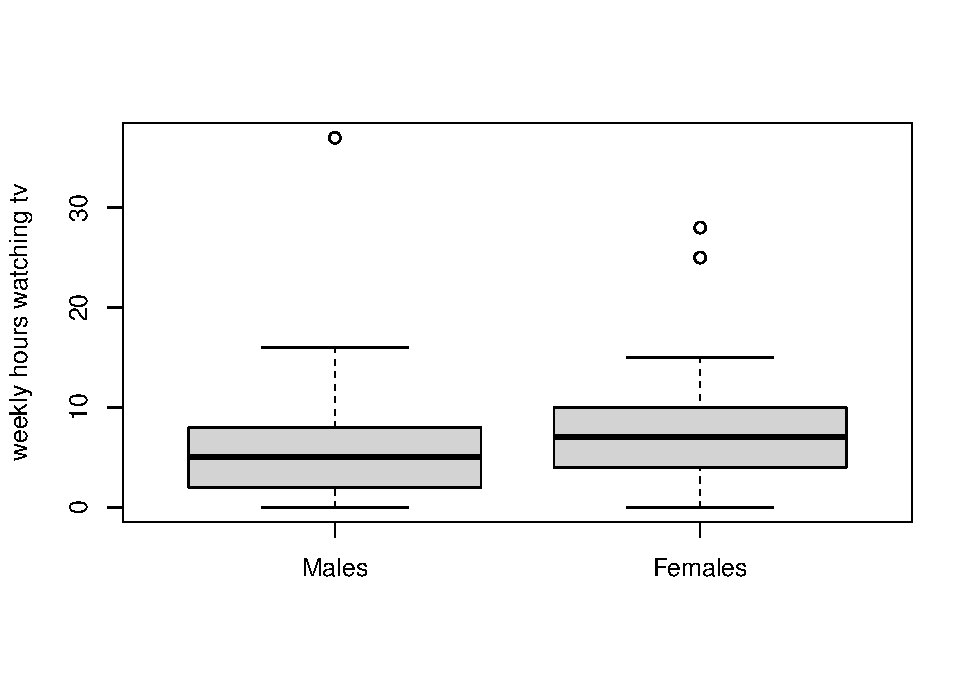
\includegraphics{Homework_1_GROUP_M_files/figure-latex/4.14-1.pdf}
assuming -independent populations -equal variances -normality
-\textgreater{} weakest assumption, barely 30 observations
--\textgreater{} use t student's distribution

\begin{Shaded}
\begin{Highlighting}[]
\NormalTok{x\_bar\_male }\OtherTok{=} \FunctionTok{mean}\NormalTok{(only\_male}\SpecialCharTok{$}\NormalTok{tv)}
\NormalTok{x\_bar\_female }\OtherTok{=} \FunctionTok{mean}\NormalTok{(only\_female}\SpecialCharTok{$}\NormalTok{tv)}
\NormalTok{s\_male }\OtherTok{=} \FunctionTok{sd}\NormalTok{(only\_male}\SpecialCharTok{$}\NormalTok{tv)}
\NormalTok{s\_female }\OtherTok{=} \FunctionTok{sd}\NormalTok{(only\_female}\SpecialCharTok{$}\NormalTok{tv)}
\NormalTok{n\_male }\OtherTok{=} \FunctionTok{length}\NormalTok{(only\_male}\SpecialCharTok{$}\NormalTok{tv)}
\NormalTok{n\_female }\OtherTok{=} \FunctionTok{length}\NormalTok{(only\_female}\SpecialCharTok{$}\NormalTok{tv)}

\CommentTok{\# assuming equal variance}
\NormalTok{s\_p }\OtherTok{=}\NormalTok{ ((n\_male }\SpecialCharTok{{-}}\DecValTok{1}\NormalTok{)}\SpecialCharTok{*}\NormalTok{(s\_male}\SpecialCharTok{\^{}}\DecValTok{2}\NormalTok{) }\SpecialCharTok{+}\NormalTok{ (n\_female }\SpecialCharTok{{-}} \DecValTok{1}\NormalTok{)}\SpecialCharTok{*}\NormalTok{(s\_female}\SpecialCharTok{\^{}}\DecValTok{2}\NormalTok{))}\SpecialCharTok{/}\NormalTok{(n\_male }\SpecialCharTok{+}\NormalTok{ n\_female }\SpecialCharTok{{-}}\DecValTok{1}\NormalTok{)}
\CommentTok{\# t = (x\_bar\_male {-} x\_bar\_female)/(s\_p*(1/n\_male + 1/n\_female))}
\NormalTok{SE\_diff }\OtherTok{=}\NormalTok{ (x\_bar\_male }\SpecialCharTok{{-}}\NormalTok{ x\_bar\_female)}\SpecialCharTok{/}\NormalTok{((s\_p}\SpecialCharTok{\^{}}\DecValTok{2}\NormalTok{)}\SpecialCharTok{*}\NormalTok{(}\DecValTok{1}\SpecialCharTok{/}\NormalTok{n\_male }\SpecialCharTok{+} \DecValTok{1}\SpecialCharTok{/}\NormalTok{n\_female))}
\NormalTok{mean\_diff }\OtherTok{=}\NormalTok{ x\_bar\_male }\SpecialCharTok{{-}}\NormalTok{ x\_bar\_female}
\NormalTok{z }\OtherTok{=} \FunctionTok{qt}\NormalTok{(}\FloatTok{0.975}\NormalTok{, n\_male }\SpecialCharTok{+}\NormalTok{ n\_female }\SpecialCharTok{{-}} \DecValTok{2}\NormalTok{)}
\NormalTok{CI\_diff }\OtherTok{=}\NormalTok{ mean\_diff }\SpecialCharTok{+} \FunctionTok{c}\NormalTok{(}\SpecialCharTok{{-}}\DecValTok{1}\NormalTok{, }\DecValTok{1}\NormalTok{)}\SpecialCharTok{*}\NormalTok{z}\SpecialCharTok{*}\NormalTok{SE\_diff}

\CommentTok{\# Test for equality of means}
\FunctionTok{t.test}\NormalTok{(only\_male}\SpecialCharTok{$}\NormalTok{tv, only\_female}\SpecialCharTok{$}\NormalTok{tv, }\AttributeTok{conf.level =} \FloatTok{0.05}\NormalTok{)}
\end{Highlighting}
\end{Shaded}

\begin{verbatim}
## 
##  Welch Two Sample t-test
## 
## data:  only_male$tv and only_female$tv
## t = -0.84995, df = 56.249, p-value = 0.399
## alternative hypothesis: true difference in means is not equal to 0
## 5 percent confidence interval:
##  -1.593836 -1.373906
## sample estimates:
## mean of x mean of y 
##  6.500000  7.983871
\end{verbatim}

We can not state that the variances are significantly different betweent
the 2 groups However the confidence interval seems to suggest that
females watch slightly more tv than males.

\begin{Shaded}
\begin{Highlighting}[]
\CommentTok{\# assuming unequal variance}
\NormalTok{SE\_diff }\OtherTok{=} \FunctionTok{sqrt}\NormalTok{((s\_male}\SpecialCharTok{\^{}}\DecValTok{2}\NormalTok{)}\SpecialCharTok{/}\NormalTok{n\_male }\SpecialCharTok{+}\NormalTok{ (s\_female}\SpecialCharTok{\^{}}\DecValTok{2}\NormalTok{)}\SpecialCharTok{/}\NormalTok{n\_female)}
\CommentTok{\# t = (x\_bar\_male {-} x\_bar\_female)/(s\_p*(1/n\_male + 1/n\_female))}
\NormalTok{mean\_diff }\OtherTok{=}\NormalTok{ x\_bar\_male }\SpecialCharTok{{-}}\NormalTok{ x\_bar\_female}
\NormalTok{z }\OtherTok{=} \FunctionTok{qt}\NormalTok{(}\FloatTok{0.975}\NormalTok{, n\_male }\SpecialCharTok{+}\NormalTok{ n\_female }\SpecialCharTok{{-}} \DecValTok{2}\NormalTok{)}
\NormalTok{CI\_diff\_uvars }\OtherTok{=}\NormalTok{ mean\_diff }\SpecialCharTok{+} \FunctionTok{c}\NormalTok{(}\SpecialCharTok{{-}}\DecValTok{1}\NormalTok{, }\DecValTok{1}\NormalTok{)}\SpecialCharTok{*}\NormalTok{z}\SpecialCharTok{*}\NormalTok{SE\_diff}
\end{Highlighting}
\end{Shaded}

Now we the interval crosses 0?? how is such a different result possible?

\hypertarget{exercise-4.16}{%
\section{Exercise 4.16}\label{exercise-4.16}}

\begin{Shaded}
\begin{Highlighting}[]
\NormalTok{data }\OtherTok{=} \FunctionTok{read.table}\NormalTok{(}\StringTok{"https://stat4ds.rwth{-}aachen.de/data/Substance.dat"}\NormalTok{, }\AttributeTok{header =} \ConstantTok{TRUE}\NormalTok{)}

\CommentTok{\# compare alcohol users and non{-}users}
\NormalTok{alpha }\OtherTok{=} \FloatTok{0.05}
\NormalTok{n }\OtherTok{=} \FunctionTok{sum}\NormalTok{(data}\SpecialCharTok{$}\NormalTok{count)}
\CommentTok{\# find the total number of students that have or haven\textquotesingle{}t used alcohol}
\NormalTok{N\_alcohol\_total }\OtherTok{=} \FunctionTok{sum}\NormalTok{(data[data}\SpecialCharTok{$}\NormalTok{alcohol }\SpecialCharTok{==} \StringTok{"yes"}\NormalTok{, }\DecValTok{4}\NormalTok{])}
\NormalTok{N\_NOalcohol\_total }\OtherTok{=} \FunctionTok{sum}\NormalTok{(data[data}\SpecialCharTok{$}\NormalTok{alcohol }\SpecialCharTok{==} \StringTok{"no"}\NormalTok{, }\DecValTok{4}\NormalTok{])}
\NormalTok{N\_marijuana }\OtherTok{=} \FunctionTok{sum}\NormalTok{(data[data}\SpecialCharTok{$}\NormalTok{alcohol }\SpecialCharTok{==} \StringTok{"yes"} \SpecialCharTok{\&}\NormalTok{ data}\SpecialCharTok{$}\NormalTok{marijuana }\SpecialCharTok{==} \StringTok{"yes"}\NormalTok{, }\DecValTok{4}\NormalTok{])}
\NormalTok{N\_NOalcohol\_marijuana }\OtherTok{=} \FunctionTok{sum}\NormalTok{(data[data}\SpecialCharTok{$}\NormalTok{alcohol }\SpecialCharTok{==} \StringTok{"no"} \SpecialCharTok{\&}\NormalTok{ data}\SpecialCharTok{$}\NormalTok{marijuana }\SpecialCharTok{==} \StringTok{"yes"}\NormalTok{, }\DecValTok{4}\NormalTok{])}

\NormalTok{pi\_1\_hat }\OtherTok{=}\NormalTok{ N\_marijuana}\SpecialCharTok{/}\NormalTok{N\_alcohol\_total}
\NormalTok{pi\_2\_hat }\OtherTok{=}\NormalTok{ N\_NOalcohol\_marijuana}\SpecialCharTok{/}\NormalTok{N\_NOalcohol\_total}

\CommentTok{\# by hand}
\NormalTok{z }\OtherTok{=} \FunctionTok{qnorm}\NormalTok{(}\DecValTok{1}\SpecialCharTok{{-}}\NormalTok{alpha}\SpecialCharTok{/}\DecValTok{2}\NormalTok{)}
\NormalTok{SE }\OtherTok{=}\NormalTok{ (pi\_1\_hat}\SpecialCharTok{*}\NormalTok{(}\DecValTok{1} \SpecialCharTok{{-}}\NormalTok{ pi\_1\_hat)}\SpecialCharTok{/}\NormalTok{N\_alcohol\_total }\SpecialCharTok{+}\NormalTok{ pi\_2\_hat}\SpecialCharTok{*}\NormalTok{(}\DecValTok{1} \SpecialCharTok{{-}}\NormalTok{ pi\_2\_hat)}\SpecialCharTok{/}\NormalTok{N\_NOalcohol\_total)}
\NormalTok{CI\_prop }\OtherTok{=}\NormalTok{ (pi\_1\_hat }\SpecialCharTok{{-}}\NormalTok{ pi\_2\_hat) }\SpecialCharTok{+} \FunctionTok{c}\NormalTok{(}\SpecialCharTok{{-}}\DecValTok{1}\NormalTok{, }\DecValTok{1}\NormalTok{)}\SpecialCharTok{*}\NormalTok{z}\SpecialCharTok{*}\FunctionTok{sqrt}\NormalTok{(SE)}

\CommentTok{\#with software}
\FunctionTok{prop.test}\NormalTok{(}\FunctionTok{c}\NormalTok{(}\DecValTok{955}\NormalTok{, }\DecValTok{5}\NormalTok{), }\FunctionTok{c}\NormalTok{(}\DecValTok{1949}\NormalTok{, }\DecValTok{327}\NormalTok{), }\AttributeTok{conf.level =}\NormalTok{ alpha, }\AttributeTok{correct =}\NormalTok{ F)}
\end{Highlighting}
\end{Shaded}

\begin{verbatim}
## 
##  2-sample test for equality of proportions without continuity
##  correction
## 
## data:  c(955, 5) out of c(1949, 327)
## X-squared = 258.73, df = 1, p-value < 2.2e-16
## alternative hypothesis: two.sided
## 5 percent confidence interval:
##  0.4738766 0.4755321
## sample estimates:
##     prop 1     prop 2 
## 0.48999487 0.01529052
\end{verbatim}

Interpretation: there seems to be a significant mean difference in the
use of marijuana between students that used alcohol before and students
who didn't.

\hypertarget{exercise-4.48}{%
\section{Exercise 4.48}\label{exercise-4.48}}

\hypertarget{given}{%
\subsection{Given}\label{given}}

\[
\text{Given } \quad SE = \sqrt{\frac{\hat{p}(1 - \hat{p})}{n}}
\]

With 95\% likelihood, find: \[ 
SE \leq \frac{1}{\sqrt{n}} \quad \text{when } \hat{p} = 0.5 
\] This is where \(SE\) is maximized.

\[
SE = \sqrt{\frac{0.5 \times (0.5)}{n}} = \frac{\sqrt{0.25}}{\sqrt{n}} = \frac{0.5}{\sqrt{n}} = \frac{1}{2 \sqrt{n}}
\]

\hypertarget{example-when-hatp-neq-0.5}{%
\subsection{\texorpdfstring{Example: When
\(\hat{p} \neq 0.5\)}{Example: When \textbackslash hat\{p\} \textbackslash neq 0.5}}\label{example-when-hatp-neq-0.5}}

\[
SE = \sqrt{\frac{0.3 \times (1 - 0.3)}{n}} = \sqrt{\frac{0.21}{n}} = \frac{0.458}{\sqrt{n}} \approx \frac{0.91}{2\sqrt{n}}
\]

\hypertarget{example-when-hatp-0.2}{%
\subsection{\texorpdfstring{Example: When
\(\hat{p} = 0.2\)}{Example: When \textbackslash hat\{p\} = 0.2}}\label{example-when-hatp-0.2}}

\[
SE = \sqrt{\frac{0.2 \times (0.8)}{n}} = \sqrt{\frac{0.16}{n}} = \frac{0.4}{\sqrt{n}} = \frac{0.8}{2\sqrt{n}}
\]

\hypertarget{example-when-hatp-0.7}{%
\subsection{\texorpdfstring{Example: When
\(\hat{p} = 0.7\)}{Example: When \textbackslash hat\{p\} = 0.7}}\label{example-when-hatp-0.7}}

\[
SE = \sqrt{\frac{0.7 \times (0.3)}{n}} = \sqrt{\frac{0.21}{n}} = \frac{0.458}{\sqrt{n}} \approx \frac{0.91}{2\sqrt{n}}
\]

\hypertarget{observation}{%
\subsection{Observation}\label{observation}}

\[
\text{Note that when both } \hat{p} < 0.5 \text{ and } \hat{p} > 0.5 \text{ the numerator decreases, along with the standard error.}
\]

\hypertarget{for-maximum-standard-error}{%
\subsection{For Maximum Standard
Error}\label{for-maximum-standard-error}}

Set the maximum \(SE\) to be within margin \(M\).

\[
\frac{1}{\sqrt{n}} = M
\]

\[
\Rightarrow \frac{1}{M} = \sqrt{n} \Rightarrow n = \frac{1}{M^2}
\]

As long as \(n \geq \frac{1}{M^2}\), our error will be within \(M\).

\hypertarget{fsds-chapter-5-exercises-5.2-5.12-5.50}{%
\subsubsection{FSDS: Chapter 5, exercises 5.2, 5.12,
5.50}\label{fsds-chapter-5-exercises-5.2-5.12-5.50}}

\begin{Shaded}
\begin{Highlighting}[]
\CommentTok{\# Placeholder for code for Exercise B5}
\end{Highlighting}
\end{Shaded}


\end{document}
